%% Normalidade Contextual em APIs -- versão 7 (regimes normais admissíveis por contexto; limite no percentil 95)
%% Classe acmart (sigconf), compatível com Overleaf (pdfLaTeX, XeLaTeX ou LuaLaTeX).
\documentclass[sigconf,nonacm]{acmart}

\usepackage[brazilian]{babel}
\usepackage{booktabs}
\usepackage{amsmath}
\usepackage{xspace}
\usepackage{fancyvrb}

\citestyle{acmauthoryear}
\settopmatter{printacmref=false, printfolios=true}
\renewcommand{\keywordsname}{Palavras-chave}
\setlength{\emergencystretch}{1.5em}

\newcommand{\Normal}{\textsc{Normal}\xspace}
\newcommand{\Residual}{\textsc{Residual}\xspace}

\begin{document}

\title{Normalidade Contextual em APIs: Regimes Normais a partir de Access Logs para Apoio à Análise de Incidentes}

\author{Diego Paz Casagrande}
\affiliation{%
  \institution{Universidade de Brasília}
  \city{Brasília}
  \state{DF}
  \country{Brasil}}

\renewcommand{\shortauthors}{D. P. Casagrande}

\begin{abstract}
Quando um incidente é aberto, uma das primeiras perguntas do operador é se as APIs envolvidas estão operando normalmente e, se não estão, qual indicador saiu do padrão. A resposta não é trivial, porque uma API tem vários comportamentos normais, que variam com o horário, o calendário e os processamentos em lote, e que mudam ao longo dos meses. Este trabalho investiga se \emph{API Access Logs} (AALs) agregados por minuto permitem identificar os múltiplos regimes normais de cada endpoint e verificar, no instante do registro do incidente, se o endpoint se enquadra em algum dos regimes admissíveis para aquele horário (\Normal) ou em nenhum deles (\Residual); qual indicador é responsável: erros de negócio (4xx), erros de sistema (5xx) ou latência; e desde quando. Seguindo o CRISP-DM, os regimes de cada endpoint são obtidos por k-means sobre o histórico, cada um com mediana e MAD próprias; um regime é admissível num contexto (tipo de dia e hora) se ocorreu nele no histórico; cada indicador tem um limite no percentil 95 dos seus desvios, calibrado por validação cruzada; e uma expansão retroativa a partir do registro, em faixas de 15~min a 4~h, estima o início do desvio. Em 5,6 milhões de registros de 12 endpoints de produção (maio a setembro de 2026), foram encontrados de 2 a 8 regimes por endpoint, com 2,7 regimes admissíveis por contexto em média. Em 12.157 consultas simuladas em agosto e setembro, o método classificou corretamente 92,5\% dos controles como \Normal e sinalizou 53,9\% dos incidentes, apontando o indicador correto em 90,4\% deles; o início real ficou dentro da zona estimada em 89,0\%. Os mesmos regimes sem a restrição de contexto detectaram significativamente menos (44,0\%), e 48\% dos controles normais se enquadraram em um regime que não é o predominante no horário. Com a mesma taxa de alarmes, o método equivale aos baselines em detecção; seu ganho está na explicação. Um histórico de 1 mês detectou mais que o de 3 meses, o que recomenda retreino frequente.
\end{abstract}

\keywords{Mineração de Dados; API Access Log; Normalidade Contextual; Regimes Operacionais; Análise de Incidentes; CRISP-DM.}

\maketitle

%% =====================================================================
\section{Introdução}

A arquitetura dos sistemas modernos consolidou o uso de APIs (\emph{Application Programming Interfaces}) como mecanismo fundamental de integração em sistemas distribuídos. Em ambientes corporativos de grande porte, as APIs medeiam desde requisições de clientes externos até transações entre sistemas legados e modernos. No Banco do Brasil, cerca de 30 mil APIs são executadas diariamente, conectando soluções de negócio que combinam plataformas em nuvem e \emph{mainframe}.

\subsection{Contexto}

Requisições processadas por gateways de API geram registros com o instante da execução, o recurso acessado, o código de resposta, o tempo de processamento e o consumidor. Neste estudo, esses registros são denominados \emph{API Access Logs} (AALs), o registro gerado pelo gateway para as requisições processadas, distinto do \emph{execution log} e do log de aplicação. Os AALs estão disponíveis de forma padronizada para um conjunto amplo de APIs, sem instrumentação específica no código.

O comportamento operacional de uma API não é necessariamente estacionário. Volume, latência e proporção de erros variam com o horário, o dia da semana, os processamentos em lote e as janelas de manutenção. Uma taxa de erros elevada pode ser normal na virada do dia, assim como latência maior pode indicar degradação ou apenas um aumento esperado de volume de requisições; uma queda abrupta de tráfego pode indicar indisponibilidade ou o fim de um período de atendimento. Uma mesma API tem, portanto, \emph{vários comportamentos normais}, e um mesmo horário pode admitir mais de um deles: à meia-noite, por exemplo, o lote pode ou não estar em execução.

\subsection{Problema}
Quando um incidente é registrado, o operador precisa contextualizar semanticamente a situação e responder, para cada API envolvida: \emph{o período anterior ao registro se enquadra em algum dos comportamentos normais esperados para aquele momento?} Se não se enquadra, também importa saber quais métricas desviaram: erros de negócio (faixa 4xx), erros de sistema (faixa 5xx) ou latência; e desde quando o desvio acontece. Como informação complementar, interessa saber se o impacto é generalizado ou concentrado em uma aplicação cliente específica com volume suficiente para alterar o estado da API; um erro espalhado entre todos os consumidores sugere um problema no provedor.

Hoje essa resposta depende de consultar várias ferramentas e de conhecer o comportamento típico de cada API e endpoint~\citep{zhang2025isre}. Abordagens com limites fixos ou com um único perfil de normalidade não distinguem a variação legítima, como um lote à meia-noite ou o volume menor no domingo, de um desvio real.

Do ponto de vista de mineração de dados, o problema consiste em: (1) identificar os regimes normais de cada recurso a partir de AALs agregados em janelas, e os contextos (tipo de dia e hora) em que cada um ocorre; (2) classificar o período imediatamente anterior ao registro de um incidente em dois estados: \Normal (enquadrado em algum regime normal admissível para aquele contexto) ou \Residual (em nenhum deles); e (3) quando \Residual, identificar qual parâmetro desviou, sendo este o indicador responsável, e desde quando.

\subsection{Motivação}
Este trabalho complementa um projeto de mestrado sobre sistemas multiagente para apoio ao atendimento de incidentes. A literatura recente mostra agentes especializados em diferentes fontes de dados, coordenados para triagem e análise~\citep{yu2025triangle,luo2025opsagent,zhang2025isre}. Um desses agentes precisa de uma fonte confiável e explicável sobre o comportamento das APIs. O foco não é monitoração em tempo real nem a identificação da causa raiz, mas a \emph{informação de contexto no instante do incidente}: dizer se cada endpoint está em um de seus regimes normais e, se não, qual indicador está impactado e desde quando. Essa informação abastece o operador por meio de um agente especialista e colabora para a análise do ocorrido, entregando um contexto semântico embasado nas atividades da mineração de dados (``o recurso está no regime de lote da meia-noite'', ``o recurso está fora dos três regimes esperados às 10h''), economizando recursos computacionais e evitando alucinações no agente, dada a quantidade de informações necessárias à análise.

\subsection{Objetivos}
\textbf{Objetivo geral:} identificar os regimes normais de cada endpoint da API a partir de Access Logs agregados por minuto e, no instante do registro de um incidente, informar se o endpoint se enquadra em algum regime normal admissível para aquele momento e, se não, qual indicador foi impactado e desde quando.

\textbf{Objetivos específicos:}
\begin{itemize}
  \item Verificar se cada endpoint apresenta vários regimes normais e em quais contextos (hora e tipo de dia) cada um ocorre.
  \item Construir, para cada regime, um perfil de normalidade e uma regra de decisão \Normal ou \Residual explicável, restrita aos regimes admissíveis no contexto.
  \item Identificar o indicador responsável (4xx, 5xx, latência) e estimar o início do desvio.
  \item Avaliar o método em cenários de incidente simulados em dois meses e compará-lo a um perfil único por contexto, aos mesmos regimes sem contexto e a baselines simples.
  \item Avaliar quanto histórico o modelo precisa (3 meses ou 1 mês).
  \item Disponibilizar a informação em formato estruturado para um agente ou operador.
\end{itemize}

\subsection{Questões de pesquisa}
\begin{itemize}
  \item \textbf{RQ1.} AALs agregados permitem identificar os regimes normais de cada recurso e decidir, no instante do registro, se o recurso se enquadra em algum deles? O contexto é necessário para essa decisão?
  \item \textbf{RQ2.} Quando o recurso não se enquadra em nenhum regime normal, o método identifica corretamente o indicador responsável (4xx, 5xx, latência) e o início do desvio?
  \item \textbf{RQ3.} Um histórico mais longo (3 meses) produz um modelo melhor do que o histórico recente (1 mês)?
\end{itemize}

\subsection{Contribuições e organização}
As contribuições são: (i) a caracterização empírica dos regimes normais de 12 recursos de API de produção ao longo de cinco meses; (ii) um método simples e explicável, sem rótulos, que representa cada recurso por vários regimes normais, restringe-os aos admissíveis em cada contexto e decide se o recurso se enquadra em algum deles no instante do registro, apontando o indicador impactado; (iii) uma estimativa de início por expansão retroativa; (iv) um protocolo de avaliação com cenários de incidente simulados em dois meses, que inclui a comparação com e sem contexto; e (v) evidência de que, nesses dados, o histórico recente é mais útil que o longo. A Seção~\ref{sec:correlatos} discute os trabalhos correlatos; a Seção~\ref{sec:metodologia}, a metodologia; a Seção~\ref{sec:resultados}, os resultados; a Seção~\ref{sec:discussao}, a discussão; a Seção~\ref{sec:ameacas}, as ameaças à validade; e a Seção~\ref{sec:conclusao} conclui.

%% =====================================================================
\section{Trabalhos correlatos}\label{sec:correlatos}

A literatura relacionada é organizada em quatro frentes e avaliada segundo quatro critérios que decorrem do problema tratado aqui: (i) a fonte de dados exigida; (ii) o tratamento dado à normalidade, isto é, se o comportamento esperado é único ou condicionado ao contexto; (iii) o tipo de saída produzida, escore ou explicação; e (iv) a necessidade de rótulos ou de instrumentação adicional. A Tabela~\ref{tab:correlatos} resume a comparação.

\begin{table*}[t]
  \caption{Comparação com os trabalhos correlatos segundo os quatro critérios.}
  \label{tab:correlatos}
  \small
  \begin{tabular}{p{0.17\textwidth}p{0.19\textwidth}p{0.17\textwidth}p{0.2\textwidth}p{0.18\textwidth}}
    \toprule
    Trabalho & Fonte de dados & Normalidade & Saída & Rótulos ou instrumentação \\
    \midrule
    DeepLog, LogAnomaly & sequências de log de sistema & única & escore ou rótulo binário & log de aplicação com \emph{templates} \\
    SPOT/DSPOT & série temporal univariada & adaptada ao longo do tempo & limiar e alarme & --- \\
    USAD & séries multivariadas & única & escore & período de treino limpo \\
    \citet{wang2025crosssystem} & \emph{traces} & única por sistema & categoria da anomalia & \emph{traces}; exemplos rotulados \\
    DeepTraLog, GAMMA & \emph{traces}, logs e métricas & única & escore ou localização & instrumentação distribuída \\
    Triangle, OpsAgent, ISRE & múltiplas fontes do incidente & não modelada (consome evidências) & triagem ou diagnóstico & integração com as fontes \\
    \midrule
    \textbf{Este trabalho} & AAL agregado por minuto & vários regimes normais, admissíveis por contexto & estado, regime, indicador e início, com explicação & nenhum além do AAL; sem rótulos \\
    \bottomrule
  \end{tabular}
\end{table*}

\subsection{Análise e mineração de logs}
\citet{du2017deeplog} propuseram o DeepLog, que modela sequências de eventos de log com redes LSTM e sinaliza como anômala toda sequência pouco provável sob o modelo aprendido. \citet{meng2019loganomaly} estenderam essa linha com o LogAnomaly, combinando a informação semântica dos \emph{templates} com a detecção de anomalias sequenciais e quantitativas. Ambos sustentam a premissa que também adotamos: logs carregam informação suficiente para caracterizar comportamento, sem instrumentação dedicada.

As diferenças, porém, são decisivas para o problema aqui tratado. Primeiro, a unidade de análise é a sequência de eventos de log de sistema, que pressupõe \emph{templates} estáveis e acesso ao log de aplicação; o AAL é um agregado por minuto, sem ordem de eventos e sem texto a partir do qual extrair \emph{templates}. Segundo, e mais importante, a normalidade nesses modelos é única: aprende-se uma distribuição de sequências normais, e o que foge dela é anômalo. Um lote à meia-noite ou uma janela de manutenção produzem padrões legítimos que um modelo sem contexto tende a tratar como desvio, a menos que o horário entre implicitamente como atributo, o que os trabalhos não exploram. Terceiro, a saída é um escore ou um rótulo binário. Para o operador que acaba de abrir um incidente, saber que a sequência é improvável não responde qual indicador saiu do padrão nem desde quando.

\subsection{Normalidade e séries temporais}
\citet{siffer2017dspot} propuseram o SPOT e sua variante com \emph{drift}, o DSPOT, que calibram limiares a partir da cauda da distribuição usando Teoria de Valores Extremos, com adaptação a séries não estacionárias. É o trabalho mais próximo do nosso em espírito: ambos reconhecem que o limiar não pode ser fixo e o derivam da própria distribuição observada, sem rótulos. O DSPOT adapta o limiar \emph{ao longo do tempo}, seguindo a série; o perfil contextual a trata como função de variáveis conhecidas \emph{a priori}, hora e tipo de dia. A consequência prática é que a adaptação temporal absorve uma degradação lenta como se fosse o novo normal, ao passo que o condicionamento por contexto preserva a referência do mesmo horário em dias anteriores. Em compensação, o DSPOT não exige que os contextos relevantes sejam conhecidos de antemão, o que é uma vantagem em domínios onde a sazonalidade não é óbvia.

\citet{audibert2020usad} propuseram o USAD, baseado em autoencoders para séries multivariadas. O método é mais expressivo que o nosso e captura dependências entre indicadores. Há ainda a questão do treinamento, que pressupõe um período limpo de anomalias; em dados de produção sem histórico de incidentes rotulado, como os nossos, essa suposição não é verificável.

\citet{wang2025crosssystem} documentam a dificuldade de transferir modelos de detecção entre sistemas distintos, mesmo com meta-aprendizado. O achado é relevante como justificativa negativa para nossa escolha de ajustar um perfil por recurso: se a transferência entre sistemas é difícil, a transferência entre recursos de perfis de tráfego muito diferentes nos nossos dados dificilmente seria mais fácil. A contrapartida é que perfis por recurso não generalizam para recursos novos, que precisam acumular histórico antes de serem avaliados; nossos resultados em setembro, com recursos de histórico curto, mostram esse custo.

\subsection{Modelagem comportamental de microsserviços}
O DeepTraLog~\citep{zhang2022deeptralog} combina \emph{traces} e logs em um grafo de eventos e aprende, com redes neurais em grafos, a estrutura esperada de uma requisição; o GAMMA~\citep{somashekar2024gamma} localiza gargalos de desempenho explorando a topologia de dependências entre serviços. Ambos entregam algo que o presente trabalho não entrega: localização, isto é, a indicação de \emph{onde} na cadeia de chamadas o problema se manifesta.

Esse ganho tem um pré-requisito. Ambos pressupõem \emph{traces} distribuídos ou métricas de infraestrutura correlacionadas, que exigem instrumentação consistente em todos os serviços da cadeia. Em ambientes corporativos heterogêneos, que combinam plataformas em nuvem e sistemas legados, essa cobertura é desigual. O AAL tem a propriedade oposta: é pobre em estrutura, porque não enxerga além do \emph{gateway}, mas é uniformemente disponível. Os dois enfoques são, portanto, complementares, e não concorrentes.

\subsection{Incidentes e sistemas multiagente}
O Triangle~\citep{yu2025triangle} organiza múltiplos agentes para a triagem de incidentes; o OpsAgent~\citep{luo2025opsagent} e o trabalho de \citet{zhang2025isre} coordenam agentes especializados em diferentes fontes para análise de incidentes e determinação de causa raiz. Esses sistemas deslocam o problema. O desafio deixa de ser o algoritmo de detecção e passa a ser a qualidade e a legibilidade das evidências que cada agente consome.

É nesse ponto que a avaliação desses trabalhos deixa uma questão em aberto. A competência do sistema multiagente é medida de ponta a ponta (acurácia de triagem, acerto de causa raiz), sem que se isole a contribuição de cada fonte nem se caracterize seu regime de erro.

\subsection{Síntese e lacuna}
A comparação revela um padrão: os trabalhos que dispensam rótulos tratam a normalidade como única ou como algo que se adapta ao longo do tempo, mas não como uma família de regimes legítimos coexistentes; os que modelam comportamento com riqueza suficiente para distinguir situações dependem de fontes além do AAL; e os que produzem explicações acionáveis o fazem no nível do sistema de agentes, assumindo como dadas as evidências que recebem. Nenhum deles investiga, exclusivamente a partir do AAL, se um mesmo recurso apresenta vários regimes normais e se essa caracterização pode informar, no instante do registro de um incidente, o estado do recurso, o indicador impactado e o início do desvio.

%% =====================================================================
\section{Metodologia}\label{sec:metodologia}

O trabalho segue o CRISP-DM~\citep{wirth2000crispdm,chapman2000crispdm}. Cada fase foi implementada em um \emph{notebook} Jupyter com parâmetros explícitos e sementes fixas (Tabela~\ref{tab:fases}). A análise é sempre por endpoint, unidade executável dentro de um produto de API. Optou-se por seis técnicas de mineração de dados no total, todas disponíveis em bibliotecas Python de uso corrente, como pandas, SciPy e scikit-learn~\citep{pedregosa2011sklearn}.

\begin{table}[t]
  \caption{Fases do CRISP-DM, notebooks e técnicas. As fases se repetem porque
  o processo é iterativo; a ordem segue a dos notebooks.}
  \label{tab:fases}
  \small
  \begin{tabular}{p{0.2\columnwidth}p{0.7\columnwidth}}
    \toprule
    Fase & Notebook: conteúdo (técnica) \\
    \midrule
    Negócio, Dados & 01: problema, critérios de sucesso, qualidade e evolução mensal da base \\
    Preparação & 02: consolidação, indicadores por janela, p95 de latência (percentil) \\
    Dados & 03: o comportamento muda com a hora? (Kruskal-Wallis com Bonferroni) \\
    Modelagem & 04: regimes normais por histórico (k-means com silhouette); perfil de cada regime (mediana/MAD); admissibilidade por contexto; limite por indicador (percentil, validação cruzada) \\
    Preparação & 05: cenários de incidente (injeção de falhas) \\
    Avaliação & 06: estado, indicador, início (expansão retroativa); histórico; IC de Wilson, McNemar \\
    Implantação & 07: consulta estruturada para o agente \\
    \bottomrule
  \end{tabular}
\end{table}

\subsection{Entendimento do negócio}
A decisão apoiada é: \emph{no instante do registro do incidente, o recurso se enquadra em algum dos seus regimes normais esperados para aquele momento? Se não, qual indicador foi impactado (erros 4xx, erros 5xx, latência) e desde quando?} A abrangência (consumidor específico ou generalizado) é informação complementar. Os critérios de sucesso foram definidos antes da modelagem (Tabela~\ref{tab:criterios}). Como não havia histórico de incidentes, a avaliação usa cenários simulados com falhas injetadas.

\subsection{Entendimento dos dados}
A base contém AALs de produção de 12 endpoints de APIs distintas, identificados aqui por E01 a E12 (em ordem decrescente de volume em agosto). Cada registro é um agregado por minuto de data e hora da execução, endpoint, código de resposta HTTP e cliente, com o total de execuções no minuto e o tempo médio dessas execuções. Como a agregação temporal por minuto já está disponível neste formato, optou-se por não utilizar os registros por execução, o que não impede que o registro bruto seja agregado da mesma forma e usado como entrada deste processo. O identificador de cliente foi anonimizado por SHA-256 com semente, sem payloads nem dados pessoais. Os horários, em UTC, foram convertidos para o horário de Brasília (UTC$-3$) antes de qualquer corte temporal.

São 5.632.001 registros de 30/04/2026 21h a 20/09/2026 20h59 (horário de Brasília), com 1.976 clientes distintos. As respostas de sucesso (2xx) somam 87,6\% das transações; os erros de negócio (4xx), 12,1\%; e os erros de sistema (5xx), 0,21\%. A cobertura varia: sete recursos têm dados desde maio; o E04, desde 25/05; cinco (E02, E03, E06, E10, E11), apenas desde 16/07; e quatro (E02, E03, E06, E11) param em 03/09. O volume mediano por hora vai de 248 transações (E11) a 9.470 (E02). Esses números mostram a heterogeneidade da base entre endpoints.

\paragraph{Evolução mensal.} O comportamento muda ao longo dos meses. Entre maio e setembro, o volume médio diário cresce de 35\% a 60\% em vários recursos (E07, E08, E12), e a taxa de erros de negócio muda de patamar: no E02, passa de 32\% (julho) para 45\% (agosto) e 62\% (setembro); no E04, de 0,5\% (maio) para 13\% (agosto). Essa mudança motiva a questão RQ3.

\subsection{Preparação dos dados}
As chaves repetidas foram consolidadas (soma do volume e média de latência ponderada). Os registros foram agregados em janelas de 1~h (29.695 janelas recurso $\times$ hora), que formam a base dos regimes. A decisão usa quatro indicadores (Tabela~\ref{tab:atributos}). O \emph{contexto} de cada janela é o par (tipo de dia, hora), com tipo de dia \emph{útil} ou \emph{não útil} (sábado, domingo e feriados: 01/05, 04/06 e 07/09).

\paragraph{Latência p95.} Como não há latência por requisição, o p95 é o percentil 95 das latências médias por minuto $\times$ cliente das respostas 2xx, ponderado pelo número de execuções. É um p95 \emph{das médias}, não das requisições, e tende a subestimar a cauda real; mas é consistente entre períodos e sensível a degradações que atingem só parte dos minutos ou dos consumidores. Na mediana, ele é 1,42 vez a latência média.

\begin{table}[t]
  \caption{Indicadores usados na decisão e direção desfavorável.}
  \label{tab:atributos}
  \small
  \begin{tabular}{p{0.2\columnwidth}p{0.52\columnwidth}p{0.16\columnwidth}}
    \toprule
    Indicador & Definição & Direção \\
    \midrule
    volume & $\log(1+$transações$)$, na escala horária & alta e queda \\
    erros 4xx & transações 4xx / total (erros de negócio) & alta \\
    erros 5xx & transações 5xx / total (erros de sistema) & alta \\
    latência p95 & $\log(1+$p95 das médias por minuto$\times$cliente$)$ & alta \\
    \bottomrule
  \end{tabular}
\end{table}

\subsection{Modelagem}

\paragraph{O comportamento muda com a hora?} O teste de Kruskal-Wallis~\citep{kruskal1952ranks}, com correção de Bonferroni~\citep{dunn1961multiple}, verifica se cada indicador muda entre as 24 horas dos dias úteis.

\paragraph{Regimes normais.} Para cada recurso e histórico, o k-means~\citep{lloyd1982kmeans} agrupa as janelas de 1~h usando apenas os quatro indicadores, padronizados e limitados aos percentis 1 e 99 do recurso, para que picos isolados não formem grupos próprios. O número de regimes, $k\in[2,8]$, é escolhido pelo coeficiente de silhouette~\citep{rousseeuw1987silhouette}, descartando as partições com algum grupo menor que 1\% das janelas. O contexto não entra no agrupamento: os regimes são definidos pelo comportamento, e a relação com o horário é aprendida depois. Cada regime recebe um nome a partir do nível de volume, dos indicadores que o distinguem (4xx, 5xx ou latência altos), do tipo de dia e das horas em que predomina; por exemplo, ``R3: volume médio, 5xx alto, dia útil, 0h''.

\paragraph{Perfil de cada regime.} Para o regime $k$ do recurso $r$ e o indicador $a$, o modelo guarda a mediana $m_a(r,k)$, a faixa p5--p95 e uma escala robusta~\citep{leys2013mad}
\begin{equation}
  s_{a}(r,k)=\max\{1{,}4826\cdot\mathrm{MAD}_{a}(r,k),\ \varepsilon_a\},
\end{equation}
em que o fator 1,4826 torna o MAD comparável ao desvio-padrão e $\varepsilon_a$ é um piso que evita divisões por valores próximos de zero. O desvio de um período $w$ em relação ao regime $k$ é
\begin{equation}
  z_a(w,k)=\frac{x_a(w)-m_a(r,k)}{s_a(r,k)},
\end{equation}
contado só no sentido desfavorável: para o volume, aumentos e quedas ($d_a=|z_a|$); para erros 4xx, erros 5xx e latência, apenas aumentos ($d_a=\max\{z_a,0\}$).

\paragraph{Admissibilidade por contexto.} Um regime é \emph{admissível} no contexto (tipo de dia, hora) se ocorreu em ao menos 5\% das janelas desse contexto no histórico, ou das horas vizinhas ($\pm$1~h), para acomodar lotes que começam um pouco antes ou depois. Assim, um mesmo horário pode admitir vários regimes normais (por exemplo, ``com lote'' e ``sem lote''), mas um regime típico da madrugada não é aceito às 10h. Contextos sem dados no histórico admitem todos os regimes.

\paragraph{Limite por indicador e decisão.} Os indicadores têm variabilidades muito diferentes; em alguns endpoints a taxa de 4xx tem picos reais frequentes. Por isso, cada indicador tem um limite próprio no recurso, $L_{r,a}=\max\{3,\ Q_{0{,}95}(d_a)\}$: o percentil 95 dos seus desvios no histórico, calculados fora da amostra. O período se \emph{enquadra} no regime $k$ se nenhum indicador passa do seu limite ($d_a(w,k)/L_{r,a}\leq 1$ para todo $a$). O período é \Normal se se enquadra em pelo menos um regime admissível no seu contexto, e \Residual caso contrário. O regime de referência é o admissível em que o período melhor se encaixa (menor $\max_a d_a/L_{r,a}$): para um período \Normal, é o regime em que ele está; para um \Residual, é o regime mais próximo, e o \textbf{indicador responsável} é o que mais passou do limite em relação a ele.

\paragraph{Histórico e calibração sem vazamento.} Para cada mês de teste (agosto; 1 a 20 de setembro), os regimes, os perfis, a admissibilidade e os limites são ajustados só com dados anteriores, em dois históricos: \emph{3 meses} (principal; maio a julho para agosto e junho a agosto para setembro) e \emph{1 mês} (o mês anterior). Os desvios fora da amostra vêm de validação cruzada com quatro blocos contíguos de tempo dentro do histórico: o modelo é ajustado em três blocos e avalia o restante. Como o regime de referência depende dos limites, a calibração é feita em duas passadas: a primeira escolhe o regime sem limites, e a segunda o escolhe com os limites da primeira e recalcula os percentis.

\paragraph{Consulta no registro e início estimado (expansão retroativa).} No instante $t$ do registro, o método olha para trás a partir de $t$ em faixas disjuntas cada vez mais distantes: 0--15, 15--30 e 30--60~min e, depois, de hora em hora até 4~h. A faixa mais recente, $[t-15\,\text{min}, t)$, define o \emph{estado no registro}, o regime de referência e o indicador responsável. Se ela for \Residual, a busca continua para trás e para na primeira faixa \Normal; o início é estimado entre o começo da última faixa residual e o fim dessa faixa normal (``começou entre 30 e 120~min antes do registro''). Todas as faixas são comparadas aos mesmos regimes de 1~h: o volume é convertido para a escala horária, e as taxas e o p95 são usados diretamente. Como faixas curtas variam mais, cada tamanho de faixa recebe seus próprios limites, calibrados da mesma forma.

\paragraph{Abrangência (complementar).} Para erros 4xx ou 5xx, o desvio é atribuído a um \emph{consumidor específico} quando o cliente com mais erros concentra ao menos 80\% deles e essa fatia supera em pelo menos 20 pontos percentuais a sua fatia do volume; caso contrário, é \emph{generalizado}. Recursos com menos de três clientes ativos ficam indeterminados.

\subsection{Avaliação}

\paragraph{Cenários de incidente.} Cada cenário simula um incidente: uma degradação começa em $t_0$ e o incidente é registrado em $t=t_0+\Delta$, com atraso $\Delta\in\{15,30,60,120\}$~min. O instante de registro é sorteado dentro do mês de teste. Entram no teste de um mês os recursos com ao menos 28 dias de dados no mês anterior: 7 recursos em agosto e os 12 em setembro. As falhas (Tabela~\ref{tab:falhas}) são aplicadas nos registros por minuto $\times$ cliente e depois reagregadas, para que os indicadores e a abrangência reajam como numa falha real. Foram gerados 5 cenários por recurso $\times$ mês $\times$ motivo $\times$ intensidade $\times$ atraso (6.080 incidentes, dos quais 3 sem tráfego foram descartados) e 6.080 consultas de controle, em instantes sem falha injetada.

\begin{table}[t]
  \caption{Motivos injetados.}
  \label{tab:falhas}
  \small
  \begin{tabular}{p{0.26\columnwidth}p{0.64\columnwidth}}
    \toprule
    Motivo & Intensidade (baixa / média / alta / muito alta) \\
    \midrule
    4xx generalizado & 5\% / 15\% / 40\% das 2xx viram 400 \\
    4xx de 1 consumidor & 30\% / 60\% / 90\% das 2xx do consumidor viram 400 \\
    5xx generalizado & 5\% / 15\% / 40\% das 2xx viram 503 \\
    5xx de 1 consumidor & 30\% / 60\% / 90\% das 2xx do consumidor viram 503 \\
    Latência & tempo de execução $\times$1,5 / $\times$2,5 / $\times$4 / $\times$10 \\
    \bottomrule
  \end{tabular}
  \par\smallskip\footnotesize O consumidor afetado é sorteado com probabilidade proporcional ao seu volume.
\end{table}

\paragraph{Latência $\times$10.} Como a latência vem de médias por minuto, poucas requisições lentas elevam muito o valor. No histórico de maio a agosto, o p95 horário ultrapassou 10 vezes a mediana do seu contexto em 0,78\% das horas (percentil 99,9: 25 vezes; máximo: 68 vezes). Degradações de latência relevantes para um incidente tendem a ser desse tamanho, por isso a intensidade ``muito alta'' ($\times$10) foi incluída para a latência. As intensidades menores foram mantidas para mostrar o limite do método.

\paragraph{Métricas.} Para cada cenário, a consulta é feita no instante do registro, como descrito acima. As métricas são: \emph{sensibilidade} (incidentes com saída \Residual); \emph{especificidade} (controles com saída \Normal); \emph{acurácia do indicador} (indicador apontado igual ao do motivo injetado, entre os detectados); \emph{acerto do início} (início real dentro da zona estimada pela expansão retroativa); e \emph{acurácia da abrangência}. ``Média/alta'' refere-se às intensidades média e alta, sem a latência $\times$10, para comparação com versões anteriores do estudo. As proporções têm intervalos de confiança de Wilson a 95\%~\citep{wilson1927probable}.

\paragraph{Comparações.} Quatro alternativas, com o mesmo tratamento de limites (percentil 95) e calibração, isolam o efeito de cada escolha. O \emph{perfil por contexto} usa um único normal por (tipo de dia, hora): mediana e MAD das janelas daquele contexto, sem regimes. Os \emph{regimes sem contexto} usam os mesmos regimes do método proposto, mas aceitam qualquer um deles a qualquer hora; a comparação mostra se a admissibilidade é necessária. O \emph{z-score global} usa uma única referência por recurso, sem contexto e sem regimes. A \emph{semana anterior} compara o período avaliado com o mesmo intervalo de tempo sete dias antes.

A comparação entre métodos usa o teste exato de McNemar~\citep{mcnemar1947note} sobre os acertos de estado nos mesmos cenários simulados. O teste considera apenas os casos em que os métodos divergem: aqueles em que o método proposto acerta e o outro erra, e aqueles em que ocorre o contrário. Um valor $p$ pequeno indica evidência de diferença estatisticamente significativa entre os métodos. Como o mesmo percentil gera taxas de alarme diferentes em cada método, eles também são comparados com a mesma meta de alarmes no histórico (1\%, 2\%, 5\% e 10\%), ajustando um multiplicador sobre os limites. O mesmo teste de McNemar compara os modelos ajustados com históricos de 3 meses e de 1 mês.

\paragraph{Experimentos.} \textbf{Exp.~1} caracteriza os regimes normais de cada recurso e sua admissibilidade por contexto. \textbf{Exp.~2} avalia o estado no registro: sensibilidade, especificidade e comparação com as alternativas. \textbf{Exp.~3} avalia a consulta quando o recurso é \Residual: indicador responsável, início estimado pela expansão retroativa e abrangência. \textbf{Exp.~4} compara os históricos de 3 meses e de 1 mês.

%% =====================================================================
\section{Resultados}\label{sec:resultados}

\subsection{Exp.~1: regimes normais por recurso}

A Figura~\ref{fig:perfis} mostra perfis horários típicos: lote na virada do dia e às 18h dos dias úteis (E01), lote às 15--16h (E05), padrão comercial em dias úteis que desaparece nos dias não úteis (E02, E12). O mapa de calor (Figura~\ref{fig:mapa}) confirma que cada recurso tem sua própria assinatura horária de volume e de latência. Nos dias úteis, 96\% dos testes de Kruskal-Wallis (recurso $\times$ indicador) foram significativos após Bonferroni. O efeito mediano ($\varepsilon^2$) foi grande para volume (0,40), erros 4xx (0,28) e latência p95 (0,25), e pequeno para erros 5xx (0,05), que em dias normais são raros.

\begin{figure*}[t]
  \centering
  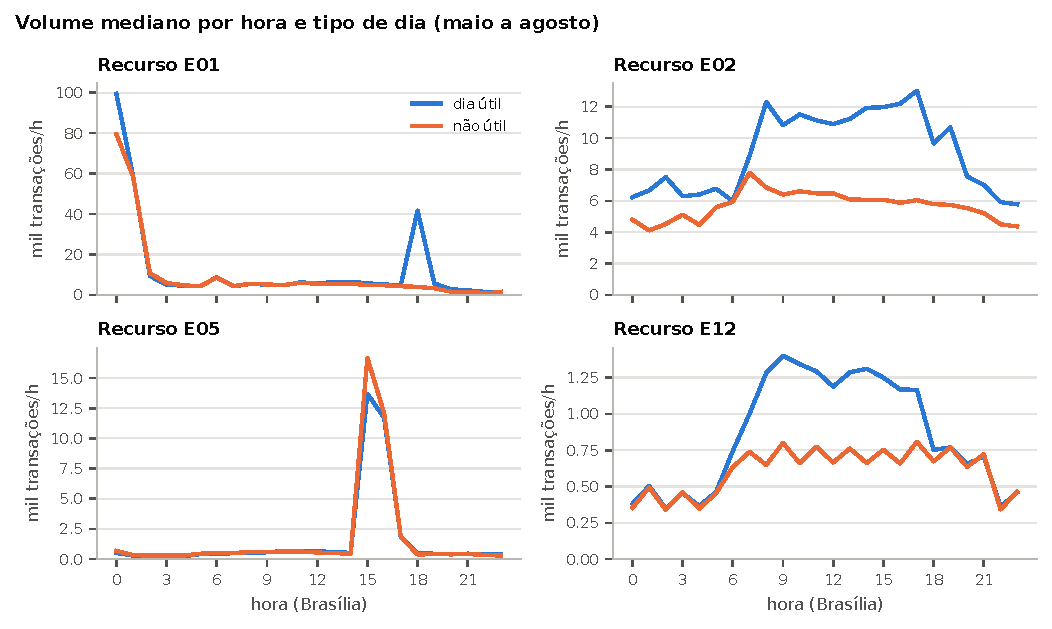
\includegraphics[width=0.9\textwidth]{figuras/fig_perfis_volume.pdf}
  \caption{Volume mediano por hora e tipo de dia (maio a agosto), em quatro recursos.}
  \label{fig:perfis}
\end{figure*}

\begin{figure*}[t]
  \centering
  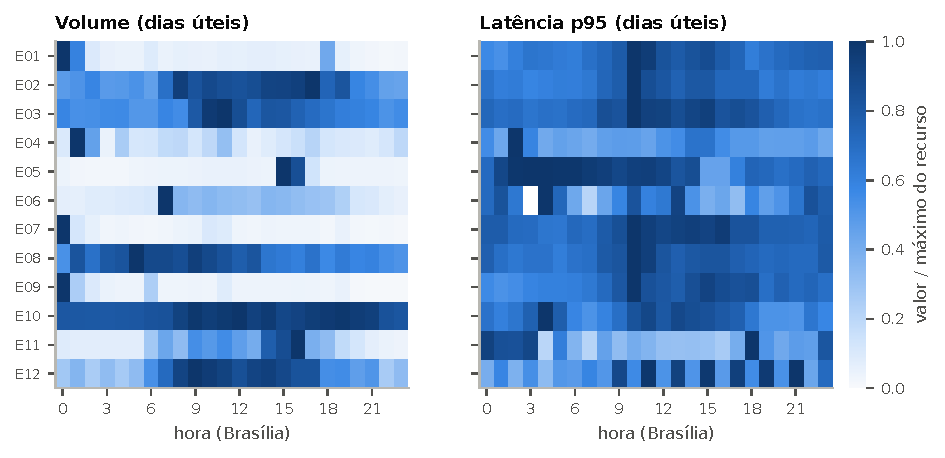
\includegraphics[width=0.85\textwidth]{figuras/fig_mapa_calor.pdf}
  \caption{Volume e latência p95 medianos por hora em dias úteis, normalizados pelo máximo de cada recurso.}
  \label{fig:mapa}
\end{figure*}

No modelo usado em setembro (histórico de junho a agosto), o k-means encontrou de 2 a 8 regimes por recurso (mediana 3,5; silhouette médio 0,51; Tabela~\ref{tab:recursos}). Em média, 2,7 regimes são admissíveis em cada contexto, e em 9 dos 12 recursos a maioria dos contextos admite mais de um regime normal. A Figura~\ref{fig:regimes} ilustra o E02. Há um regime de volume alto que ocupa as 8 às 17h dos dias úteis, regimes de volume baixo e médio fora do horário comercial, um regime de volume alto com latência alta, que aparece de forma esporádica ao longo do dia, e o regime ``R3: volume médio, 5xx alto'', que só ocorre à 0h. Esse último é \emph{normal} no lote da meia-noite e só é admissível entre 23h e 1h: um 5xx elevado às 10h não se enquadra nele. Nos dias não úteis, quase todos os regimes são admissíveis em quase todas as horas, porque há poucas janelas por contexto e o comportamento varia mais.

\begin{figure*}[t]
  \centering
  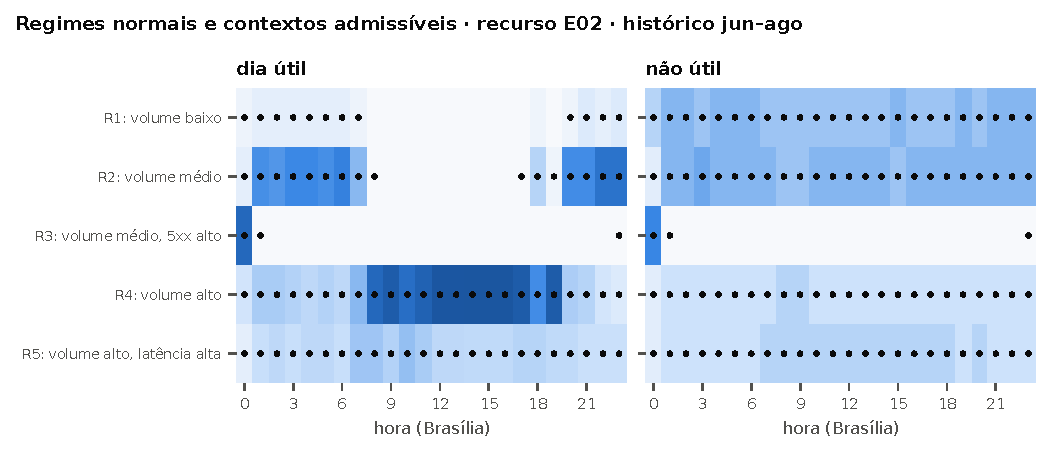
\includegraphics[width=0.85\textwidth]{figuras/fig_regimes_admissiveis.pdf}
  \caption{Regimes normais do recurso E02 (histórico de junho a agosto): fração das janelas de cada contexto em cada regime (cor) e contextos em que o regime é admissível (pontos).}
  \label{fig:regimes}
\end{figure*}

\begin{table*}[t]
  \caption{Resumo por recurso: participação no volume, clientes, transações medianas por hora, regimes e regimes admissíveis por contexto (Exp.~1, modelo de setembro), meses de teste e resultados da consulta no registro (Exp.~2 e 3, histórico de 3 meses).}
  \label{tab:recursos}
  \small
  \setlength{\tabcolsep}{4.5pt}
  \begin{tabular}{lrrrrrrcrrrr}
    \toprule
    Recurso & Vol. (\%) & Clientes & Trans./h & Regimes ($k$) & Silhouette & Admiss./contexto & Teste & Sensib. & Sensib. média/alta & Especif. & Acurácia indicador \\
    \midrule
    E01 & 47,3 & 38  & 5.120 & 5 & 0,39 & 3,6 & ago, set & 0,68 & 0,73 & 0,93 & 0,96 \\
    E02 & 11,9 & 555 & 9.470 & 5 & 0,55 & 3,7 & set & 0,34 & 0,38 & 0,85 & 0,60 \\
    E03 & 3,1  & 246 & 2.535 & 4 & 0,52 & 2,6 & set & 0,31 & 0,37 & 0,95 & 0,86 \\
    E04 & 4,9  & 24  & 925   & 2 & 0,60 & 1,5 & ago, set & 0,60 & 0,66 & 0,88 & 0,83 \\
    E05 & 6,0  & 19  & 483   & 2 & 0,75 & 1,3 & ago, set & 0,78 & 0,82 & 0,92 & 0,97 \\
    E06 & 2,4  & 787 & 1.583 & 2 & 0,64 & 1,1 & set & 0,12 & 0,09 & 0,94 & 0,74 \\
    E07 & 5,7  & 36  & 596   & 2 & 0,61 & 1,4 & ago, set & 0,55 & 0,62 & 0,96 & 0,97 \\
    E08 & 5,9  & 39  & 1.128 & 5 & 0,36 & 3,5 & ago, set & 0,57 & 0,63 & 0,93 & 0,91 \\
    E09 & 5,6  & 30  & 578   & 3 & 0,62 & 2,1 & ago, set & 0,68 & 0,73 & 0,93 & 0,91 \\
    E10 & 2,2  & 2   & 1.038 & 8 & 0,29 & 6,0 & set & 0,25 & 0,26 & 0,98 & 0,86 \\
    E11 & 1,9  & 625 & 248   & 3 & 0,55 & 2,7 & set & 0,30 & 0,33 & 0,93 & 0,63 \\
    E12 & 2,9  & 831 & 723   & 4 & 0,29 & 3,0 & ago, set & 0,60 & 0,68 & 0,92 & 0,95 \\
    \bottomrule
  \end{tabular}
\end{table*}

\subsection{Limites por indicador}
Com o percentil 95, a maioria dos limites fica no piso de $z=3$ (Figura~\ref{fig:limites}): os desvios em relação ao regime de referência são pequenos, porque cada regime já agrupa comportamentos parecidos. Limites acima do piso revelam indicadores que variam muito mesmo dentro dos regimes: erros 4xx em E04 (35) e E07 (12), latência p95 em E02 (12) e volume em E05 e E09 (5). No histórico de junho a agosto, fora da amostra, 7,4\% das janelas de 1~h ficaram fora de todos os regimes admissíveis, com erros 4xx (534 janelas), volume (464), latência (407) e erros 5xx (150) como indicadores responsáveis.

\begin{figure}[t]
  \centering
  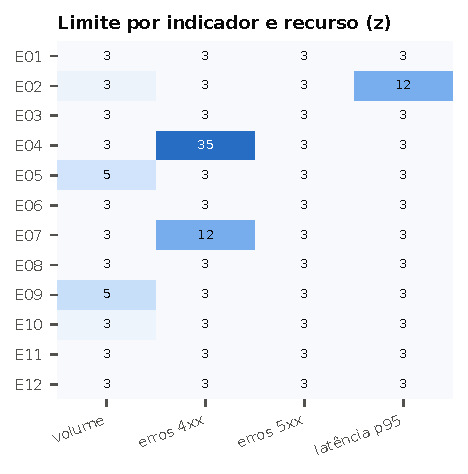
\includegraphics[width=0.75\columnwidth]{figuras/fig_limites.pdf}
  \caption{Limite de cada indicador por recurso ($z$ em relação ao regime de referência, percentil 95 fora da amostra, mínimo 3) nas janelas de 1~h; histórico de junho a agosto.}
  \label{fig:limites}
\end{figure}

\subsection{Exp.~2: estado no instante do registro}
A Tabela~\ref{tab:metodos} e a Figura~\ref{fig:metodos} resumem a decisão. O método proposto classificou corretamente 92,5\% dos controles como \Normal e sinalizou como \Residual 53,9\% dos incidentes (58,6\% nas intensidades média e alta).

\paragraph{O contexto é necessário.} Os mesmos regimes sem a restrição de contexto detectaram muito menos (44,0\%; McNemar $p<0{,}001$ a favor do método proposto). Sem a admissibilidade, um período degradado encontra com frequência algum regime de outro horário em que se encaixa: um 5xx elevado às 10h, por exemplo, cabe no regime do lote da meia-noite. A perda é maior justamente onde os regimes de outro horário se parecem com a falha: erros 4xx generalizados (28\% contra 46\%) e latência (35\% contra 45\%).

\paragraph{Múltiplos regimes por contexto.} Em 78\% das consultas, o contexto do registro tinha mais de um regime admissível (2,7 em média), e 48\% dos controles classificados como \Normal se enquadraram em um regime que \emph{não} é o predominante naquele horário. Um perfil único por contexto teria de acomodar esses casos alargando a sua faixa normal.

\begin{table*}[t]
  \caption{Exp.~2: estado no registro por método, com o limite no percentil 95, em \% (IC de Wilson a 95\% entre colchetes). Histórico de 3 meses; 6.077 incidentes e 6.080 controles. $p$: McNemar dos acertos de estado contra o método proposto (entre parênteses, quem acerta mais).}
  \label{tab:metodos}
  \small
  \begin{tabular}{lccccc}
    \toprule
    Método & Sensibilidade & Sensibilidade (média/alta) & Especificidade & Acurácia do indicador & $p$ \\
    \midrule
    \textbf{Regimes normais (proposto)} & \textbf{53,9} [52,7; 55,2] & \textbf{58,6} [57,1; 60,2] & \textbf{92,5} [91,8; 93,1] & \textbf{90,4} [89,4; 91,4] & --- \\
    Perfil por contexto & 61,7 [60,5; 62,9] & 66,9 [65,3; 68,3] & 88,7 [87,9; 89,5] & 93,0 [92,2; 93,8] & $<$0,001 (perfil) \\
    Regimes sem contexto & 44,0 [42,7; 45,2] & 48,4 [46,8; 50,0] & 95,6 [95,0; 96,0] & 88,5 [87,2; 89,6] & $<$0,001 (proposto) \\
    z-score global & 58,8 [57,5; 60,0] & 63,2 [61,6; 64,7] & 91,4 [90,7; 92,1] & 94,0 [93,2; 94,8] & $<$0,001 (z-score) \\
    Semana anterior & 59,0 [57,8; 60,2] & 64,1 [62,6; 65,6] & 91,3 [90,6; 92,0] & 94,4 [93,6; 95,1] & $<$0,001 (semana) \\
    \bottomrule
  \end{tabular}
\end{table*}

\begin{figure*}[t]
  \centering
  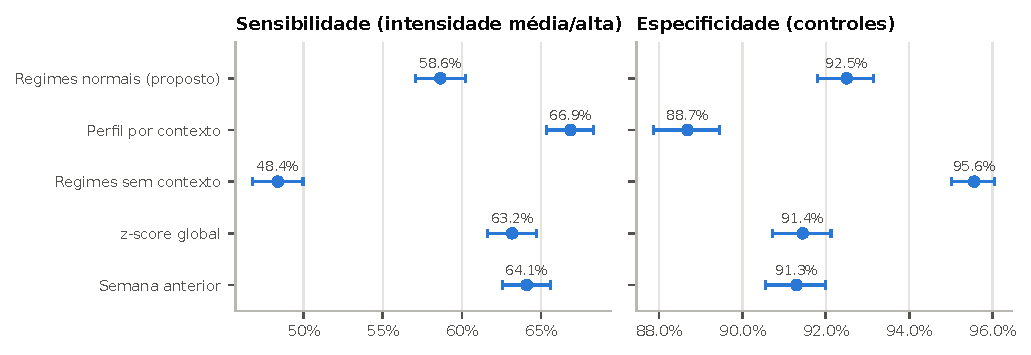
\includegraphics[width=0.85\textwidth]{figuras/fig_metodos.pdf}
  \caption{Sensibilidade (intensidades média e alta) e especificidade por método, com o limite no percentil 95 e IC de Wilson a 95\%.}
  \label{fig:metodos}
\end{figure*}

\paragraph{Ponto de operação.} Com o mesmo percentil, os métodos operam em pontos diferentes: o método proposto alarma menos (7,5\% dos controles) que o perfil por contexto (11,3\%), o z-score global (8,6\%) e a semana anterior (8,7\%), e por isso detecta menos. No teste de McNemar no ponto adotado, os três acertam mais estados que o método proposto. A comparação justa é com a mesma meta de alarmes (Figura~\ref{fig:curva}, Tabela~\ref{tab:operacao}). Nesse caso, os métodos com contexto ficam próximos entre si: com 1\% de alarmes, o método proposto detecta um pouco mais (25,6\% contra 22,9\% a 23,8\%); com 5\%, fica entre eles (46,9\% contra 46,1\% a 48,1\%). Os regimes sem contexto ficam abaixo em todos os pontos.

\begin{figure}[t]
  \centering
  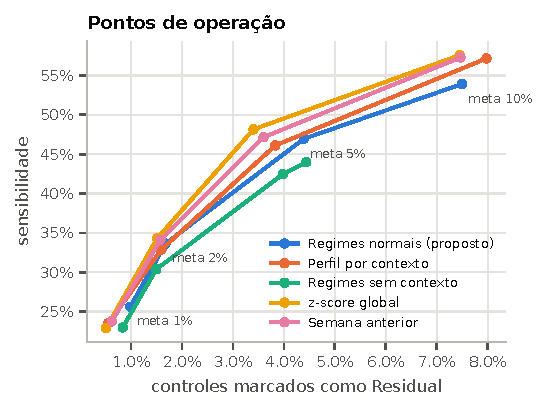
\includegraphics[width=0.85\columnwidth]{figuras/fig_curva_operacao.pdf}
  \caption{Curva de operação: sensibilidade contra controles marcados como \Residual, para metas de 1\%, 2\%, 5\% e 10\% de alarmes no histórico.}
  \label{fig:curva}
\end{figure}

\begin{table}[t]
  \caption{Sensibilidade / especificidade (\%) com a mesma meta de alarmes no histórico.}
  \label{tab:operacao}
  \small
  \begin{tabular}{lccc}
    \toprule
    Método & Meta 1\% & Meta 2\% & Meta 5\% \\
    \midrule
    \textbf{Regimes normais} & \textbf{25,6} / 99,0 & 33,6 / 98,3 & 46,9 / 95,6 \\
    Perfil por contexto & 23,5 / 99,4 & 32,9 / 98,4 & 46,1 / 96,2 \\
    Regimes sem contexto & 23,0 / 99,2 & 30,4 / 98,5 & 42,5 / 96,0 \\
    z-score global & 22,9 / 99,5 & 34,3 / 98,5 & 48,1 / 96,6 \\
    Semana anterior & 23,8 / 99,4 & 34,1 / 98,4 & 47,2 / 96,4 \\
    \bottomrule
  \end{tabular}
\end{table}

\paragraph{Por motivo.} A sensibilidade depende fortemente do motivo (Figura~\ref{fig:sensmotivo}). Erros de sistema generalizados são detectados em 66\% a 91\% dos casos, conforme a intensidade, e erros 5xx de um consumidor em 56\% a 69\%. Erros de negócio têm detecção de 33\% a 63\% (generalizados) e de 29\% a 46\% (um consumidor). A latência vai de 13\% ($\times$1,5) a 58\% ($\times$4) e chega a \textbf{79\%} [74; 83] na degradação de 10 vezes. A sensibilidade varia pouco com o atraso entre o início da degradação e o registro: de 57\% a 61\% nas intensidades média e alta.

\begin{figure}[t]
  \centering
  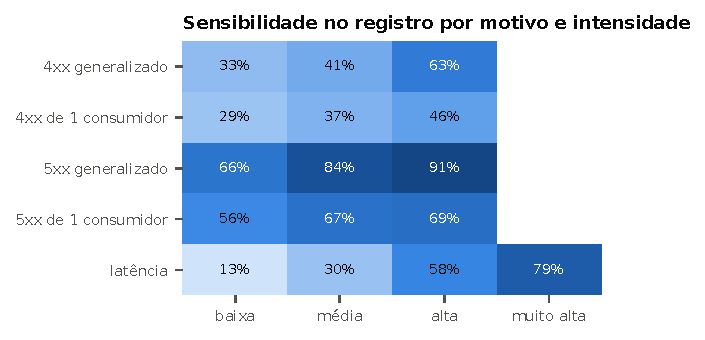
\includegraphics[width=0.9\columnwidth]{figuras/fig_sens_motivo.pdf}
  \caption{Sensibilidade no registro do método proposto, por motivo e intensidade.}
  \label{fig:sensmotivo}
\end{figure}

\paragraph{Por recurso e por mês.} Por recurso (Tabela~\ref{tab:recursos}), a sensibilidade vai de 12\% (E06) a 78\% (E05). Por mês, a sensibilidade foi de 62,2\% em agosto (7 recursos) e 49,1\% em setembro (12 recursos); restrita aos mesmos 7 recursos, setembro teve 65,4\%. A queda de setembro vem, portanto, dos recursos que só entram nesse mês, com menos histórico e mais variação.

\subsection{Exp.~3: indicador responsável, início e abrangência}
Quando o recurso é sinalizado como \Residual, o indicador apontado em relação ao regime mais próximo é o do motivo injetado em 90,4\% dos casos [89,4; 91,4] (Figura~\ref{fig:confusao}): 96,4\% para 5xx generalizado, 94,5\% para 5xx de um consumidor, 84,9\% para latência e 85--86\% para 4xx. O erro mais comum é apontar o volume (9--10\% dos casos de 4xx e de latência): como o regime mais próximo é escolhido entre vários, às vezes é um regime de volume diferente que melhor acomoda o indicador degradado. A acurácia é menor em E02 (60\%) e E11 (63\%), recursos com muita variação natural em outros indicadores.

\begin{figure}[t]
  \centering
  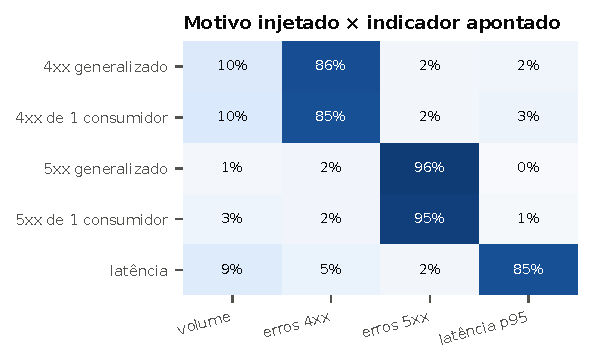
\includegraphics[width=0.85\columnwidth]{figuras/fig_confusao_indicador.pdf}
  \caption{Motivo injetado contra indicador apontado (casos detectados).}
  \label{fig:confusao}
\end{figure}

A Figura~\ref{fig:expansao} ilustra a expansão retroativa em um cenário de 5xx generalizado iniciado 60~min antes do registro. As três faixas mais recentes são residuais (4,7 a 6,1 vezes o limite) e a de 60--120~min é normal; o início é estimado entre 30 e 120~min antes do registro e contém o início real. Nos casos detectados, o início real ficou dentro da zona estimada em 89,0\% [87,9; 90,1] (Tabela~\ref{tab:consulta}): 96\% e 98\% quando a degradação começou 15 ou 30~min antes do registro, 83\% com 60~min e 78\% com 120~min (Figura~\ref{fig:inicio}). Os erros são quase sempre subestimações: uma faixa intermediária sai \Normal, a busca para cedo e o início é estimado mais perto do registro do que de fato ocorreu.

\begin{figure*}[t]
  \centering
  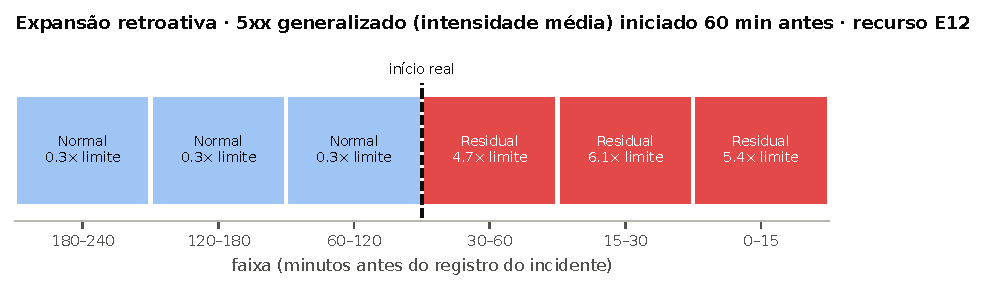
\includegraphics[width=0.85\textwidth]{figuras/fig_expansao_exemplo.pdf}
  \caption{Expansão retroativa em um cenário de 5xx generalizado iniciado 60~min antes do registro (E12): as três faixas mais recentes são residuais e a de 60--120~min é normal, e o início é estimado entre 30 e 120~min antes.}
  \label{fig:expansao}
\end{figure*}

\begin{figure}[t]
  \centering
  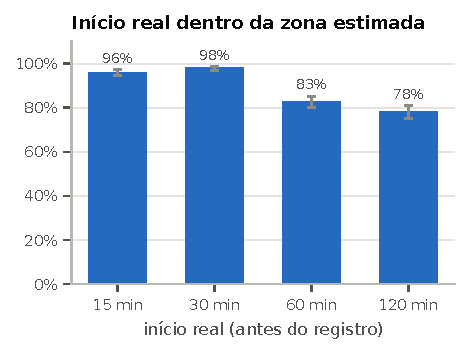
\includegraphics[width=0.8\columnwidth]{figuras/fig_inicio.pdf}
  \caption{Início real dentro da zona estimada, por atraso entre o início da degradação e o registro (IC de Wilson a 95\%).}
  \label{fig:inicio}
\end{figure}

\paragraph{Abrangência (complementar).} Entre os erros 4xx e 5xx detectados com o indicador correto, a abrangência foi classificada corretamente em 76,5\% [74,8; 78,2]. Os erros generalizados são reconhecidos como tais em 87--88\% dos casos; os de um consumidor, em 57\% (4xx) e 66\% (5xx).

\begin{table}[t]
  \caption{Exp.~3: qualidade da consulta nos incidentes detectados (método proposto, histórico de 3 meses), em \% (IC de Wilson a 95\%).}
  \label{tab:consulta}
  \small
  \begin{tabular}{lcc}
    \toprule
    Informação & Casos & Acerto \\
    \midrule
    Indicador responsável & 3.277 & 90,4 [89,4; 91,4] \\
    Início na zona estimada & 3.277 & 89,0 [87,9; 90,1] \\
    \quad degradação 15 ou 30~min antes & 1.679 & 97,1 \\
    \quad degradação 60 ou 120~min antes & 1.598 & 80,6 \\
    Abrangência (4xx e 5xx) & 2.383 & 76,5 [74,8; 78,2] \\
    \bottomrule
  \end{tabular}
\end{table}

\paragraph{Saída para o agente.} A consulta produz um documento estruturado que inclui os regimes admissíveis no contexto e o regime de referência. A Figura~\ref{fig:json} mostra, resumida, a saída do cenário da Figura~\ref{fig:expansao}. Para um período \Normal, a saída indica o regime em que ele se enquadra, por exemplo ``R6: volume alto'', um dos 4 admissíveis às 20h de um dia não útil.

\begin{figure}[t]
\begin{Verbatim}[fontsize=\scriptsize,frame=single]
{"recurso": "E12", "registro_incidente": "2026-08-02 16:52",
 "contexto": {"tipo_dia": "não útil", "hora": "16h"},
 "regimes_admissiveis": ["R2: volume baixo", "R4: volume médio",
    "R5: volume alto", "R6: volume alto",
    "R7: volume alto, latência alta"],
 "estado": "Residual", "regime_mais_proximo": "R6: volume alto",
 "indicador_impactado": "erros 5xx",
 "evidencias": [{"indicador": "erros 5xx", "observado": "16.5%",
    "faixa_normal_p5_p95": ["0.0%", "2.3%"], "vezes_o_limite": 5.43}],
 "inicio_estimado": "entre 30 e 120 min antes do registro",
 "abrangencia": {"classificacao": "generalizado",
    "clientes_ativos": 27, "clientes_com_erro": 11},
 "motivo_estatistico": "O recurso E12 está fora dos 5 regimes
   normais admissíveis para não útil às 16h; o mais próximo é
   R6: volume alto. Indicador impactado: erros 5xx — 16.5% nos
   15 min anteriores ao registro (faixa normal do regime 0.0% a
   2.3%), 5.43× o limite do recurso. O desvio começou entre 30
   e 120 min antes do registro. Os erros aparecem em 11 de 27
   consumidores ativos."}
\end{Verbatim}
\caption{Saída da consulta para o agente (resumida; nomes dos regimes encurtados).}
\label{fig:json}
\end{figure}

\paragraph{Evento real.} Nos dados reais, sem injeção, a consulta para o E02 às 01h45 de 02/09 (4,1\% de erros 5xx em 15 dos 26 consumidores ativos, um candidato a incidente real) retornou \Normal: o período se enquadrou no regime ``R3: volume médio, 5xx alto'', o do lote da meia-noite, que é admissível à 1h por causa da tolerância de $\pm$1~h. Com um único perfil por contexto, o mesmo evento é \Residual. A saída, ainda assim, é informativa: diz ao operador que o recurso se comporta como no lote da meia-noite, uma hora e quarenta e cinco minutos depois do horário habitual. Mas o caso mostra o custo da tolerância perto de regimes com erros elevados.

\subsection{Exp.~4: histórico de 3 meses $\times$ 1 mês}
O histórico mais longo \emph{não} melhorou a detecção (Tabela~\ref{tab:historico}, Figura~\ref{fig:historico}). Com 1 mês, a sensibilidade subiu de 53,9\% para 60,7\% e a especificidade caiu de 92,5\% para 88,9\%; nos acertos de estado, o histórico de 1 mês foi melhor (McNemar: $p<0{,}001$). Nos dois meses de teste, o histórico de 1 mês detectou mais (agosto: 67,5\% contra 62,2\%; setembro: 56,7\% contra 49,1\%) e alarmou mais (agosto: 88,3\% contra 92,1\% de especificidade; setembro: 89,3\% contra 92,7\%). Os limites refletem a mudança de comportamento: com 3 meses, o limite de latência do E02 fica 3,9 vezes maior, o de 4xx do E07, 2,5 vezes, e o de volume do E09, 2,1 vezes.

\begin{table}[t]
  \caption{Exp.~4: histórico de 3 meses $\times$ 1 mês (método proposto, em \%; m/a = intensidades média e alta).}
  \label{tab:historico}
  \small
  \begin{tabular}{lcccc}
    \toprule
    Histórico & Sensib. & Sensib. m/a & Especif. & Acur. indicador \\
    \midrule
    3 meses & 53,9 & 58,6 & 92,5 & 90,4 \\
    1 mês & 60,7 & 65,8 & 88,9 & 90,0 \\
    \bottomrule
  \end{tabular}
\end{table}

\begin{figure*}[t]
  \centering
  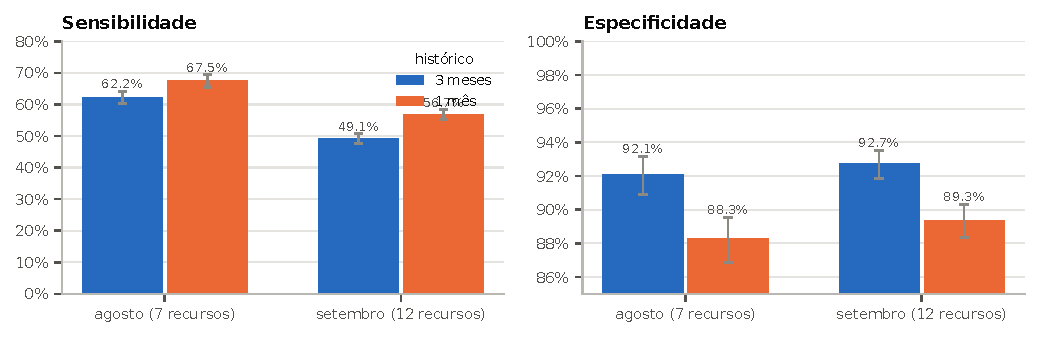
\includegraphics[width=0.85\textwidth]{figuras/fig_historico.pdf}
  \caption{Sensibilidade e especificidade por mês de teste e histórico, com IC de Wilson a 95\%.}
  \label{fig:historico}
\end{figure*}

\subsection{Critérios de sucesso}
Dois dos cinco critérios definidos no entendimento do negócio foram atendidos (Tabela~\ref{tab:criterios}): a acurácia do indicador e o acerto do início. A especificidade ficou abaixo da meta, por efeito do percentil 95, e a sensibilidade também. No ponto adotado, os baselines acertam mais estados; com a mesma meta de alarmes, os métodos se equivalem.

\begin{table}[t]
  \caption{Critérios de sucesso definidos antes da modelagem (histórico de 3 meses).}
  \label{tab:criterios}
  \small
  \begin{tabular}{p{0.5\columnwidth}p{0.22\columnwidth}c}
    \toprule
    Critério & Resultado & Atendido \\
    \midrule
    Controles com saída \Normal $\geq$ 95\% & 92,5\% & não \\
    Sensibilidade (média/alta) $\geq$ 70\% & 58,6\% & não \\
    Acurácia do indicador $\geq$ 90\% & 90,4\% & sim \\
    Início real na zona estimada $\geq$ 70\% & 89,0\% & sim \\
    Sem perda significativa para os baselines & perda no ponto adotado; empate com a mesma meta de alarmes & não \\
    \bottomrule
  \end{tabular}
\end{table}

%% =====================================================================
\section{Discussão}\label{sec:discussao}

\paragraph{RQ1: regimes e estado no registro.} Os AALs agregados mostram regimes claros: lotes na virada do dia e à tarde, horário comercial em dias úteis, madrugada e até regimes normais com erros elevados em horários específicos. Esses regimes são usados de fato na decisão. A maioria dos contextos admite mais de um regime, e quase metade dos controles normais se enquadrou em um regime que não é o predominante no horário. O resultado mais claro desta versão é que \emph{o contexto é necessário}: os mesmos regimes, aceitos a qualquer hora, detectam significativamente menos, porque um período degradado quase sempre encontra algum regime de outro horário que o acomoda. A combinação de regimes com admissibilidade por contexto é, portanto, o que dá sentido à pergunta ``o momento do incidente se enquadra em algum dos normais?''. Em detecção, porém, o método não supera as alternativas com contexto: com a mesma meta de alarmes, ele empata com o perfil por contexto, o z-score global e a semana anterior. Sua contribuição está na \emph{explicação}: ele diz em qual regime o recurso está, quais regimes seriam esperados e qual a faixa normal do regime mais próximo.

\paragraph{O ponto de operação pesa mais que o método.} Com o percentil 95, todos os métodos detectam mais e alarmam mais do que com o percentil 99. No percentil 99, o perfil por contexto tinha 39\% de sensibilidade e 97\% de especificidade; no percentil 95, tem 62\% e 89\%. As diferenças entre métodos com o mesmo percentil vêm sobretudo de cada um operar em um ponto diferente da curva. Para o uso pretendido, em que a consulta só é feita quando já existe um incidente aberto, a escolha do ponto de operação deve partir do custo de um falso \Residual para o operador.

\paragraph{O limite por indicador.} Em relação ao regime de referência, a maioria dos indicadores tem desvios pequenos, e os limites caem no piso de $z=3$. Os limites altos que restam (4xx em E04 e E07, latência em E02) apontam indicadores instáveis mesmo dentro de um regime. Isso é, por si, uma informação útil ao operador.

\paragraph{RQ2: indicador e início.} A informação emitida continua boa: o indicador responsável é apontado corretamente em 90\% dos casos, e o início é localizado na zona certa em 89\%. A acurácia do indicador caiu em relação a um perfil único por contexto (93\%), porque o regime mais próximo às vezes é um regime de volume diferente, e a diferença de volume passa a ser o maior desvio. A expansão retroativa é simples de explicar (``olhar para trás até encontrar um período normal''): faixas curtas perto do registro dão precisão quando a degradação é recente, e faixas de 1~h mais para trás estendem o horizonte até 4~h. Para o operador, um resultado \Residual vem com o indicador certo, o regime que era esperado e uma estimativa de início. Um resultado \Normal diz em qual regime o recurso está, mas não descarta degradações sutis.

\paragraph{Admissibilidade: generosa demais em alguns casos.} Dois efeitos aparecem nos dados. Primeiro, nos dias não úteis há poucas janelas por contexto, e quase todos os regimes se tornam admissíveis em quase todas as horas. Segundo, a tolerância de $\pm$1~h, criada para lotes que atrasam, absorveu o evento real do E02 à 1h45 no regime do lote da meia-noite. Os dois efeitos reduzem a sensibilidade e indicam ajustes naturais: um número mínimo de janelas por contexto, a tolerância apenas para regimes sem erros elevados, ou a admissibilidade ponderada pela frequência do regime no contexto.

\paragraph{RQ3: quanto histórico.} Mais histórico não significou um modelo melhor. As APIs mudam de patamar ao longo dos meses (volume crescendo, taxas de erro de negócio mudando), e um histórico de três meses inclui regimes que já não valem, o que alarga os regimes e os limites. Para a implantação, isso favorece o \emph{retreino frequente com o histórico recente}, por exemplo mensal com o último mês, em vez de acumular meses.

\paragraph{Latência e erros de negócio.} O p95 das médias por minuto tem caudas pesadas mesmo em dias normais (0,78\% das horas passam de 10 vezes a mediana do contexto). A latência é detectada em 79\% dos casos com a degradação de 10 vezes e em 58\% com 4 vezes, mas pouco nas degradações moderadas. Um percentil por requisição, se disponível no gateway, é o caminho natural de melhoria. Erros de negócio de um único consumidor continuam os mais difíceis: em recursos com 4xx naturais altos, há quase sempre algum regime admissível com 4xx parecido.

%% =====================================================================
\section{Ameaças à validade}\label{sec:ameacas}

\paragraph{Falhas sintéticas.} O desempenho mede a capacidade de detectar \emph{os motivos injetados}, e não falhas reais. As intensidades variadas, os quatro atrasos, os dois meses e o grande número de cenários reduzem, mas não eliminam, esse viés. A acurácia do indicador, do início e da abrangência é medida apenas sobre incidentes detectados, que tendem a ser os mais fortes.

\paragraph{Decisões tomadas ao longo do estudo.} O método de regimes admissíveis, o percentil 95 e os parâmetros de admissibilidade (5\% das janelas, $\pm$1~h) foram definidos depois de versões anteriores deste estudo, que usaram os mesmos cenários de teste; nenhum desses parâmetros foi otimizado nos cenários, e os resultados desfavoráveis são relatados. O multiplicador dos limites foi fixado em 1, porque uma meta de alarmes no histórico desfaria a escolha do percentil; os pontos com metas de 1\% a 10\% são relatados. A intensidade de latência $\times$10 é justificada pela distribuição do histórico.

\paragraph{Estabilidade dos regimes.} O k-means é refeito a cada histórico, e o número de regimes pode mudar entre meses e entre as dobras da validação cruzada. Os regimes de recursos com $k=2$ tendem a separar um padrão raro, como o lote; o tamanho mínimo de 1\% das janelas e a limitação aos percentis 1 e 99 reduzem, mas não eliminam, essa instabilidade.

\paragraph{Controles e anomalias reais.} As consultas de controle usam dados reais sem injeção, que podem conter anomalias reais, contadas como falso \Residual. A especificidade é, portanto, uma estimativa conservadora.

\paragraph{Cobertura desigual.} Cinco recursos só têm dados a partir de 16/07 e entram apenas no teste de setembro, quatro deles até 03/09; nesses, o ``histórico de 3 meses'' tem na prática cerca de seis semanas. Os feriados considerados foram 01/05, 04/06 (Corpus Christi, tratado como não útil) e 07/09.

\paragraph{Latência aproximada.} O p95 é calculado sobre as médias por minuto e por cliente, e não sobre requisições; a cauda real tende a ser maior. Uma latência 10 vezes maior poderia, na prática, esbarrar no \emph{timeout} do gateway e virar erro 504, o que a injeção não simula.

\paragraph{Anonimização e generalização.} Esta base usa outra semente de anonimização que a base de agosto usada em versões anteriores do estudo: os volumes coincidem no período comum, mas os clientes não podem ser cruzados entre as duas. Os resultados vêm de uma organização e de 12 recursos. A base não pode ser compartilhada; o código dos notebooks é independente dos dados.

%% =====================================================================
\section{Considerações finais}\label{sec:conclusao}

Este trabalho mostrou que Access Logs agregados por minuto, sem \emph{traces} nem logs de aplicação, permitem identificar os múltiplos regimes normais de cada recurso de API e verificar, no instante em que um incidente é aberto, se o recurso se enquadra em algum dos regimes admissíveis para aquele horário e, se não, qual indicador foi impactado (erros de negócio, erros de sistema ou latência) e desde quando. O método usa técnicas simples (k-means, mediana, MAD, percentis, validação cruzada e uma busca retroativa), não exige rótulos e produz uma explicação que um agente ou operador pode usar diretamente: o regime em que o recurso está, os regimes esperados e a faixa normal de cada indicador.

Em dois meses de teste, com o limite no percentil 95, o método teve 92,5\% de especificidade e 53,9\% de sensibilidade, com 90,4\% de acerto no indicador e 89,0\% na zona de início. Os regimes só funcionam com a restrição de contexto: sem ela, a detecção cai de forma significativa. Com a mesma taxa de alarmes, o método empata com um perfil único por contexto e com baselines simples; seu valor está na explicação baseada em regimes. O histórico recente (1 mês) detectou mais que o longo (3 meses), o que recomenda retreino frequente.

Como trabalhos futuros, destacam-se: (i) refinar a admissibilidade, com número mínimo de janelas por contexto, tolerância apenas para regimes sem erros elevados e pesos pela frequência do regime no contexto; (ii) validar o método com incidentes reais, começando pelo evento observado no E02, e com a avaliação de operadores; (iii) testar históricos deslizantes mais curtos e com pesos maiores para o período recente; (iv) melhorar a sensibilidade à latência com percentis por requisição; e (v) integrar a consulta como ferramenta de um agente de apoio a incidentes.

\bibliographystyle{ACM-Reference-Format}
\bibliography{referencias}

\end{document}
